\chapter{Untersuchung des Laufzeitverhaltens}
Die Untersuchung der Laufzeitverhaltens wurde mithilfe eines Logik-
Analysers durchgeführt. Ein Logikanalyser misst wie lange und wann
ein Pin 1 und/oder 0 ist. Die Pins, die nötig sind um diese Messungen
durchzuführen, dürfen noch nicht belegt sein. Vorteilhafterweise
besitzt die Platine zwei Ports, die noch nicht belegt sind aber
trotzdem nach draußen gelegt wurden, somit konnte der Logik-
Analyser an die Platine angeschlossen und ein kleines Modul
geschrieben werden, um diese Pins setzen und wieder löschen zu
können. Diese Operationen wurden als Makros implementiert um den
Messoverhead so gering wie möglich zu halten.
\begin{table}[htb]
\begin{center}
	\begin{tabular}{|c||c|c|}
		\hline
		\textbf{Makro} & \textbf{benötigte Takte} & \textbf{benötigte Zeit bei 16 MHz} \\ \hline \hline
		pin\_set() & 2 & 125 ns \\ \hline
		pin\_clear() & 2 & 125 ns \\ \hline
		pin\_toggle() & 4 & 250 ns \\ \hline
	\end{tabular}
	\caption{\label{pin_takte} Benötigte Takte/Zeit für Pin-Operationen}
\end{center}
\end{table}
Wie hier beschrieben sind die Zeiten für das Ausführen der Instruktion
zum setzen, löschen und umschalten von einzelnen Pins ziemlich gering.
Doch bei den Messungen insbesondere mit einem Leistungsfähigen und
sehr genauen Oszilloskop konnte herausgefunden werden, dass das eigentliche
Wechsel des Stroms am Pin verhältnismäßig langsam durchgeführt wird,
insbesondere das Abfallen des Stromes, also bei einer fallenden Flanke
benötigt ungefähr 2 us von denen allerdings, und hier liegt das Problem,
zwischen 0.5 und 1 us fälschlicherweise als ''high'' gemessen wird.
D.h. der Logikanalyser misst eine gewisse Zeitspanne einen ''falschen'' Wert.
(Er ist nicht physikalisch falsch nur logisch). Denn wenn der Strom abfällt
ist der bin schon nicht mehr gesetzt, der Logikanalyser allerdings betrachtet
dies teilweise immer noch als gesetzt.
Aufgrund dieses Umstandes als auch der Tatsache, dass das System nicht untersucht
werden kann ohne einen geringen Fußabdruck zu hinterlassen, sind die Messungen mit
einem abschätzbaren aber nicht genau vorhersagbaren Fehler im Vergleich zur
Wirklichkeit behaftet.
\section{Erste Messungen}
Durch die ersten Messungen wurde der Startpunkt für die Untersuchung der Software
festgelegt. Dafür wurde in der Hauptschleife (siehe Abb. \ref{main_loop_full}) zum einen
ein pin\_toggle() eingebaut, um die Länge einer Schleifeniteration zu messen, zum anderen
wurde die einzelnen Funktionsaufrufe in der Hauptschleife mit pin\_set() und pin\_clear()
umgeben.
\begin{figure}[htb]
 \centering
 \scalebox{0.5}{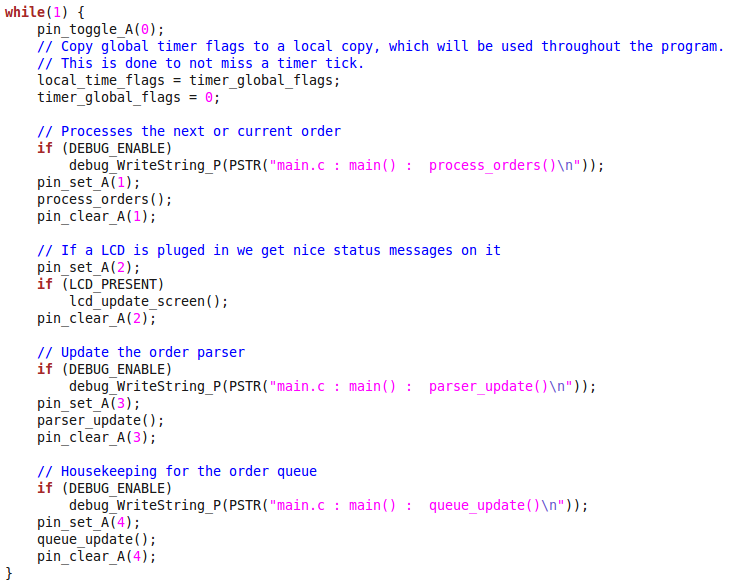
\includegraphics{pictures/main_loop_full.png}}
 \caption{\label{main_loop_full}Die Hauptschleife mit Debugausgaben und Pin-Operationen}
\end{figure}
\begin{table}[htb]
\begin{center}
	\begin{tabular}{|c||r|c|}
		\hline
		\textbf{Funktion} & \textbf{Zeit} & \textbf{Rahmenbedingungen} \\ \hline \hline
		Hauptschleife & 27,916 \textmu{}s & Idle, LCD an, DEBUG aus, I2C an, AB:EIT \\ \hline
		process\_orders() & 11,964 \textmu{}s &  \\ \hline
		lcd\_update\_screen() & 3,988 \textmu{}s &  \\ \hline
		parser\_update() & 3,988 \textmu{}s &  \\ \hline
		queue\_update() & 3,988 \textmu{}s &  \\ \hline \hline
		Hauptschleife & 47,856 \textmu{}s & ABS aktiv im Idle Status, ansonsten wie oben \\ \hline
		process\_orders() & 31,904 \textmu{}s &  \\ \hline
		lcd\_update\_screen() & 3,988 \textmu{}s &  \\ \hline
		parser\_update() & 3,988 \textmu{}s &  \\ \hline
		queue\_update() & 3,988 \textmu{}s &  \\ \hline \hline
		I2C-Bus ISR & 4,586 \textmu{}s & Adresse empfangen \\ \hline
		I2C-BUS ISR & 21,934 \textmu{}s & Daten empfangen \\ \hline
		100ms ISR & 8,076 \textmu{}s & \\ \hline \hline
		Hauptschleife & 718,843 \textmu{}s & LCD aus, Byte in Parser, Befehl bereit \\ \hline
		process\_orders() & 39,880 \textmu{}s & I2C ISR (Daten) aufgetreten \\ \hline
		lcd\_update\_screen() & 0,997 \textmu{}s &  \\ \hline
		parser\_update() & 175,474 \textmu{}s &  \\ \hline
		queue\_update() & 505,484 \textmu{}s &  \\ \hline \hline
		Hauptschleife & 718,843 \textmu{}s & LCD an, Befehl in Queue, aber nicht gestartet \\ \hline
		process\_orders() & 358,923 \textmu{}s &  \\ \hline
		lcd\_update\_screen() & 3250,000 \textmu{}s &  \\ \hline
		parser\_update() & 6,032 \textmu{}s &  \\ \hline
		queue\_update() & 5,583 \textmu{}s &  \\ \hline
	\end{tabular}
	\caption{\label{erste_messung} Ergebnisse der ersten Messungen}
\end{center}
\end{table}

\section{Das LCD-Problem}
\section{Optimierung}
\subsection{Inlining von Funktionen}
\subsection{Eleminierung von Modulo-Operatoren}
\subsection{Effizienteres Initialisieren des Speichers}
\subsection{Bedingtes Kompilieren von Debugausgaben}
\section{Vergleich mit der Original-Software}
